% ═══════════════════════════════════════════════════════════════
% Figure: MIRAGE-UAS Defense Architecture — 4-Layer Deception
% Usage: % ═══════════════════════════════════════════════════════════════
% Figure: MIRAGE-UAS Defense Architecture — 4-Layer Deception
% Usage: % ═══════════════════════════════════════════════════════════════
% Figure: MIRAGE-UAS Defense Architecture — 4-Layer Deception
% Usage: % ═══════════════════════════════════════════════════════════════
% Figure: MIRAGE-UAS Defense Architecture — 4-Layer Deception
% Usage: \input{figures/fig_defense_arch.tex}
% ═══════════════════════════════════════════════════════════════
\begin{figure*}[t]
\centering
\resizebox{\textwidth}{!}{%
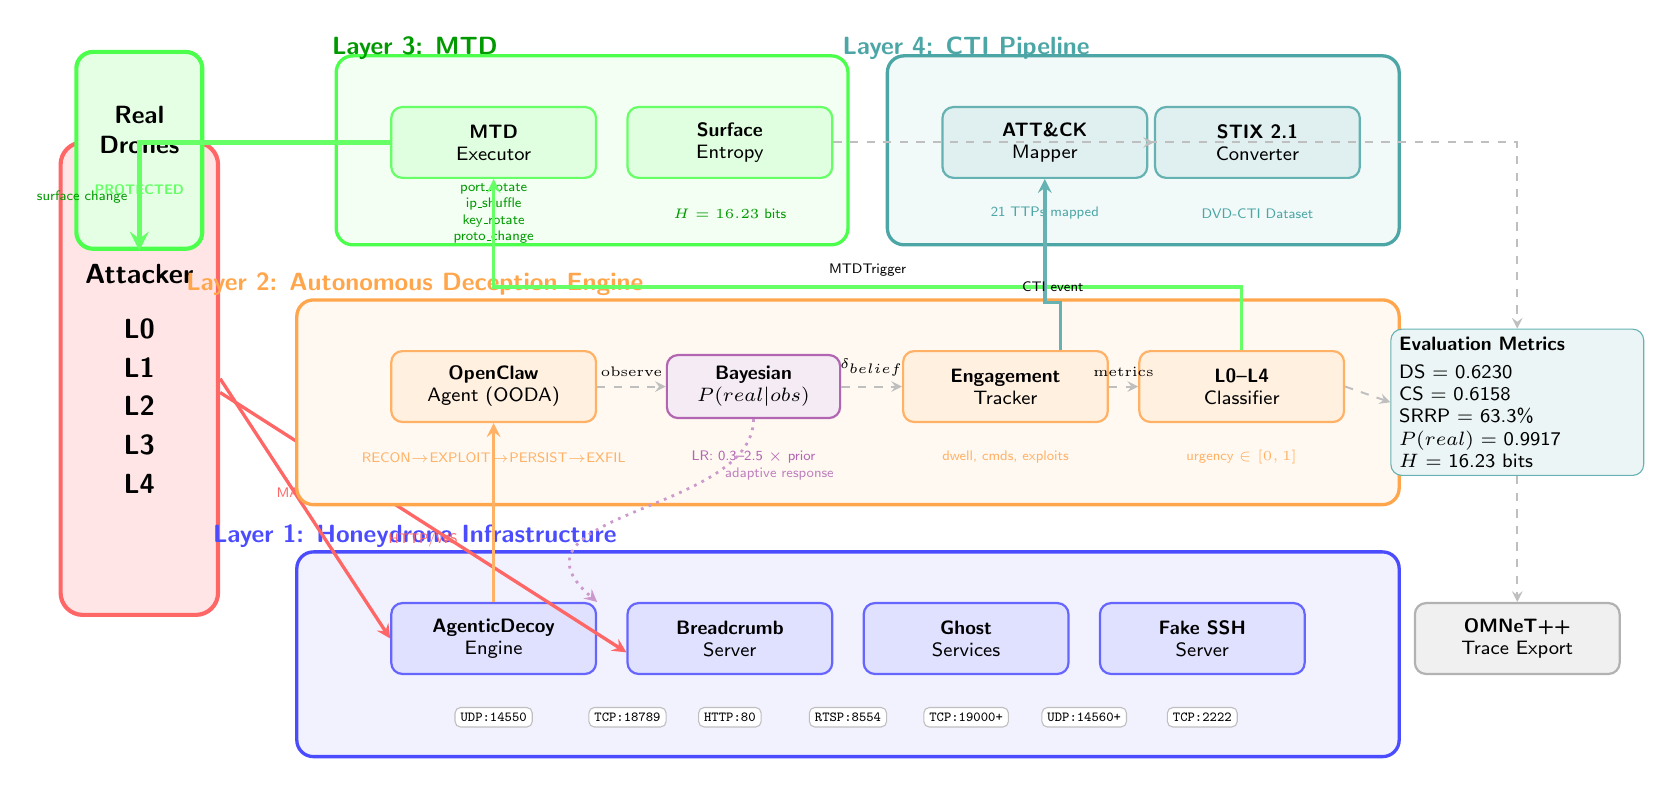
\begin{tikzpicture}[
    >=stealth,
    layer/.style={
        rectangle, rounded corners=6pt, draw=#1!70, fill=#1!5,
        line width=1.2pt, minimum height=2.8cm, align=center
    },
    comp/.style={
        rectangle, rounded corners=4pt, draw=#1!60, fill=#1!12,
        line width=0.8pt, minimum width=2.6cm, minimum height=0.9cm,
        align=center, font=\sffamily\scriptsize
    },
    port/.style={
        rectangle, rounded corners=2pt, draw=gray!50, fill=white,
        font=\ttfamily\tiny, inner sep=2pt
    },
    flow/.style={->, line width=1.2pt, draw=#1!60},
    dataflow/.style={->, line width=0.7pt, draw=gray!50, dashed},
    beliefbox/.style={
        rectangle, rounded corners=4pt, draw=violet!60, fill=violet!8,
        line width=0.8pt, font=\sffamily\scriptsize, align=center,
        minimum width=2.2cm, minimum height=0.8cm
    },
    metricbox/.style={
        rectangle, rounded corners=4pt, draw=teal!60, fill=teal!8,
        font=\sffamily\scriptsize, align=left, text width=3.0cm,
        inner sep=3pt
    },
]

% ═══════════════════════════════════════════════════════════════
% ATTACKER (left side)
% ═══════════════════════════════════════════════════════════════
\node[rectangle, rounded corners=8pt, draw=red!60, fill=red!10,
      line width=1.5pt, minimum width=2.0cm, minimum height=6cm,
      align=center, font=\sffamily\bfseries]
    (ATK) at (-2, 4.5) {Attacker\\[8pt]\romark{L0}\\[2pt]\romark{L1}\\[2pt]\romark{L2}\\[2pt]\romark{L3}\\[2pt]\romark{L4}};

% ═══════════════════════════════════════════════════════════════
% LAYER 1: Honeydrone Infrastructure (bottom)
% ═══════════════════════════════════════════════════════════════
\node[layer=blue, minimum width=14cm, minimum height=2.6cm] (L1) at (7, 1) {};
\node[font=\sffamily\bfseries\small, text=blue!70] at (1.5, 2.5) {Layer 1: Honeydrone Infrastructure};

% Components
\node[comp=blue] (engine) at (2.5, 1.2) {\textbf{AgenticDecoy}\\Engine};
\node[comp=blue] (bread)  at (5.5, 1.2) {\textbf{Breadcrumb}\\Server};
\node[comp=blue] (ghost)  at (8.5, 1.2) {\textbf{Ghost}\\Services};
\node[comp=blue] (ssh)    at (11.5, 1.2) {\textbf{Fake SSH}\\Server};

% Ports
\node[port] at (2.5, 0.2) {UDP:14550};
\node[port] at (4.2, 0.2) {TCP:18789};
\node[port] at (5.5, 0.2) {HTTP:80};
\node[port] at (7.0, 0.2) {RTSP:8554};
\node[port] at (8.5, 0.2) {TCP:19000+};
\node[port] at (10.0, 0.2) {UDP:14560+};
\node[port] at (11.5, 0.2) {TCP:2222};

% Attack arrows into Layer 1
\draw[flow=red] (ATK.east) -- node[above, font=\sffamily\tiny, text=red!60] {MAVLink} (engine.west);
\draw[flow=red] ([yshift=-5pt]ATK.east) -- node[below, font=\sffamily\tiny, text=red!60] {HTTP/WS} ([yshift=-5pt]bread.west);

% ═══════════════════════════════════════════════════════════════
% LAYER 2: Autonomous Deception (middle)
% ═══════════════════════════════════════════════════════════════
\node[layer=orange, minimum width=14cm, minimum height=2.6cm] (L2) at (7, 4.2) {};
\node[font=\sffamily\bfseries\small, text=orange!70] at (1.5, 5.7) {Layer 2: Autonomous Deception Engine};

\node[comp=orange] (ooda) at (2.5, 4.4) {\textbf{OpenClaw}\\Agent (OODA)};
\node[beliefbox]   (belief) at (5.8, 4.4) {\textbf{Bayesian}\\$P(\text{real}|\text{obs})$};
\node[comp=orange] (track) at (9.0, 4.4) {\textbf{Engagement}\\Tracker};
\node[comp=orange] (class) at (12.0, 4.4) {\textbf{L0--L4}\\Classifier};

% Subdetails
\node[font=\sffamily\tiny, text=orange!60] at (2.5, 3.5) {RECON$\to$EXPLOIT$\to$PERSIST$\to$EXFIL};
\node[font=\sffamily\tiny, text=violet!60] at (5.8, 3.5) {LR: 0.3--2.5 $\times$ prior};
\node[font=\sffamily\tiny, text=orange!60] at (9.0, 3.5) {dwell, cmds, exploits};
\node[font=\sffamily\tiny, text=orange!60] at (12.0, 3.5) {urgency $\in [0,1]$};

% Internal flows
\draw[flow=orange] (engine.north) -- (ooda.south);
\draw[dataflow] (ooda) -- node[above, font=\tiny] {observe} (belief);
\draw[dataflow] (belief) -- node[above, font=\tiny] {$\delta_{\text{belief}}$} (track);
\draw[dataflow] (track) -- node[above, font=\tiny] {metrics} (class);

% ═══════════════════════════════════════════════════════════════
% LAYER 3: MTD (top-left)
% ═══════════════════════════════════════════════════════════════
\node[layer=green, minimum width=6.5cm, minimum height=2.4cm] (L3) at (3.75, 7.4) {};
\node[font=\sffamily\bfseries\small, text=green!60!black] at (1.5, 8.7) {Layer 3: MTD};

\node[comp=green] (executor) at (2.5, 7.5) {\textbf{MTD}\\Executor};
\node[comp=green] (entropy) at (5.5, 7.5) {\textbf{Surface}\\Entropy};

\node[font=\sffamily\tiny, text=green!60!black, align=center] at (2.5, 6.6) {port\_rotate\\ip\_shuffle\\key\_rotate\\proto\_change};
\node[font=\sffamily\tiny, text=green!60!black] at (5.5, 6.6) {$H=16.23$ bits};

% MTD trigger from classifier
\draw[flow=green] (class.north) -- ++(0, 0.8) -| node[near start, above, font=\sffamily\tiny] {MTDTrigger} (executor.south);

% ═══════════════════════════════════════════════════════════════
% LAYER 4: CTI Pipeline (top-right)
% ═══════════════════════════════════════════════════════════════
\node[layer=teal, minimum width=6.5cm, minimum height=2.4cm] (L4) at (10.75, 7.4) {};
\node[font=\sffamily\bfseries\small, text=teal!70] at (8.5, 8.7) {Layer 4: CTI Pipeline};

\node[comp=teal] (parser) at (9.5, 7.5) {\textbf{ATT\&CK}\\Mapper};
\node[comp=teal] (stix)   at (12.2, 7.5) {\textbf{STIX 2.1}\\Converter};

\node[font=\sffamily\tiny, text=teal!70] at (9.5, 6.6) {21 TTPs mapped};
\node[font=\sffamily\tiny, text=teal!70] at (12.2, 6.6) {DVD-CTI Dataset};

% CTI flow
\draw[flow=teal] ([xshift=20pt]track.north) -- ++(0, 0.6) -| node[near start, above, font=\sffamily\tiny] {CTI event} (parser.south);
\draw[dataflow] (parser) -- (stix);

% ═══════════════════════════════════════════════════════════════
% METRICS OUTPUT (right side)
% ═══════════════════════════════════════════════════════════════
\node[metricbox] (metrics) at (15.5, 4.2) {
    \textbf{Evaluation Metrics}\\[2pt]
    DS = 0.6230\\
    CS = 0.6158\\
    SRRP = 63.3\%\\
    $P(\text{real})$ = 0.9917\\
    $H$ = 16.23 bits
};
\draw[dataflow] (class.east) -- (metrics.west);
\draw[dataflow] (entropy.east) -| (metrics.north);

% ═══════════════════════════════════════════════════════════════
% OMNeT++ Output (bottom-right)
% ═══════════════════════════════════════════════════════════════
\node[comp=gray] (omnet) at (15.5, 1.2) {\textbf{OMNeT++}\\Trace Export};
\draw[dataflow] (metrics.south) -- (omnet.north);

% ═══════════════════════════════════════════════════════════════
% REAL DRONES (protected, far left)
% ═══════════════════════════════════════════════════════════════
\node[rectangle, rounded corners=6pt, draw=green!70, fill=green!10,
      line width=1.5pt, minimum width=1.6cm, minimum height=2.5cm,
      align=center, font=\sffamily\bfseries\small]
    (REAL) at (-2, 7.4) {Real\\Drones\\[4pt]{\tiny\textcolor{green!60}{PROTECTED}}};

\draw[flow=green, line width=2pt] (executor.west) -| node[near end, left, font=\sffamily\tiny, text=green!60!black] {surface change} (REAL.south);

% ═══════════════════════════════════════════════════════════════
% Deception feedback loop (big curved arrow)
% ═════════════════════════════════════════════════════════���═════
\draw[->, line width=1pt, draw=violet!40, dotted]
    (belief.south) .. controls (5.8, 2.8) and (2.5, 2.8) .. (engine.north east)
    node[near start, right, font=\sffamily\tiny, text=violet!50] {adaptive response};

\end{tikzpicture}
}
\caption{MIRAGE-UAS 4-Layer 방어 아키텍처. 공격자 트래픽은 Layer~1의 허니드론 인프라에 유입되고, Layer~2의 자율 기만 엔진이 OODA 루프와 베이지안 믿음 추적으로 적응형 응답을 생성한다. Layer~3의 MTD는 공격자 레벨 기반 urgency에 따라 공격 표면을 재구성하며, Layer~4의 CTI 파이프라인은 공격 이벤트를 STIX 2.1 데이터셋으로 변환한다.}
\label{fig:defense}
\end{figure*}

% ═══════════════════════════════════════════════════════════════
\begin{figure*}[t]
\centering
\resizebox{\textwidth}{!}{%
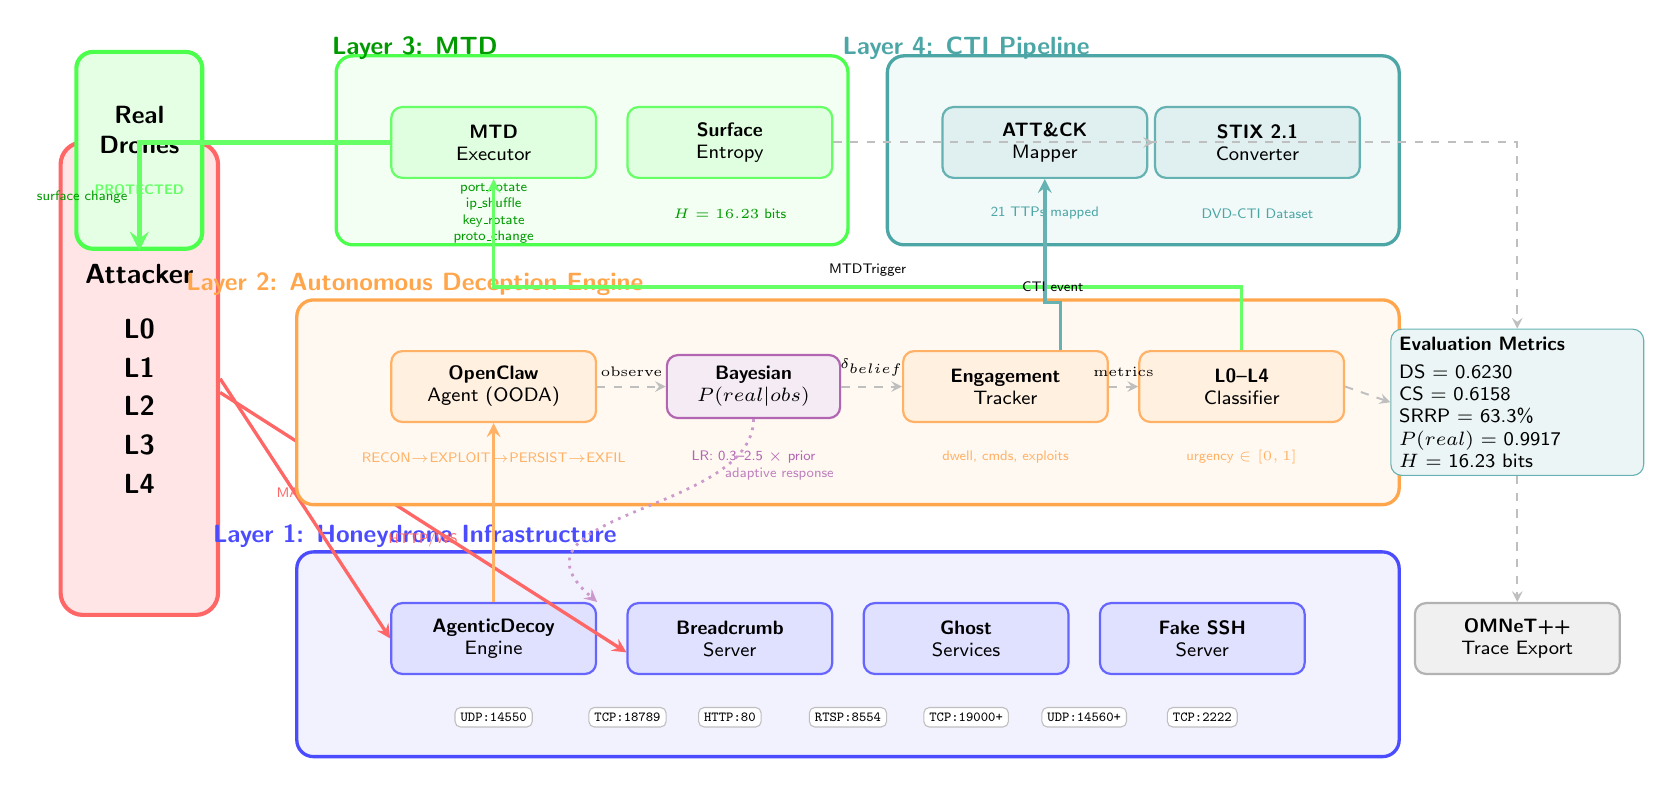
\begin{tikzpicture}[
    >=stealth,
    layer/.style={
        rectangle, rounded corners=6pt, draw=#1!70, fill=#1!5,
        line width=1.2pt, minimum height=2.8cm, align=center
    },
    comp/.style={
        rectangle, rounded corners=4pt, draw=#1!60, fill=#1!12,
        line width=0.8pt, minimum width=2.6cm, minimum height=0.9cm,
        align=center, font=\sffamily\scriptsize
    },
    port/.style={
        rectangle, rounded corners=2pt, draw=gray!50, fill=white,
        font=\ttfamily\tiny, inner sep=2pt
    },
    flow/.style={->, line width=1.2pt, draw=#1!60},
    dataflow/.style={->, line width=0.7pt, draw=gray!50, dashed},
    beliefbox/.style={
        rectangle, rounded corners=4pt, draw=violet!60, fill=violet!8,
        line width=0.8pt, font=\sffamily\scriptsize, align=center,
        minimum width=2.2cm, minimum height=0.8cm
    },
    metricbox/.style={
        rectangle, rounded corners=4pt, draw=teal!60, fill=teal!8,
        font=\sffamily\scriptsize, align=left, text width=3.0cm,
        inner sep=3pt
    },
]

% ═══════════════════════════════════════════════════════════════
% ATTACKER (left side)
% ═══════════════════════════════════════════════════════════════
\node[rectangle, rounded corners=8pt, draw=red!60, fill=red!10,
      line width=1.5pt, minimum width=2.0cm, minimum height=6cm,
      align=center, font=\sffamily\bfseries]
    (ATK) at (-2, 4.5) {Attacker\\[8pt]\romark{L0}\\[2pt]\romark{L1}\\[2pt]\romark{L2}\\[2pt]\romark{L3}\\[2pt]\romark{L4}};

% ═══════════════════════════════════════════════════════════════
% LAYER 1: Honeydrone Infrastructure (bottom)
% ═══════════════════════════════════════════════════════════════
\node[layer=blue, minimum width=14cm, minimum height=2.6cm] (L1) at (7, 1) {};
\node[font=\sffamily\bfseries\small, text=blue!70] at (1.5, 2.5) {Layer 1: Honeydrone Infrastructure};

% Components
\node[comp=blue] (engine) at (2.5, 1.2) {\textbf{AgenticDecoy}\\Engine};
\node[comp=blue] (bread)  at (5.5, 1.2) {\textbf{Breadcrumb}\\Server};
\node[comp=blue] (ghost)  at (8.5, 1.2) {\textbf{Ghost}\\Services};
\node[comp=blue] (ssh)    at (11.5, 1.2) {\textbf{Fake SSH}\\Server};

% Ports
\node[port] at (2.5, 0.2) {UDP:14550};
\node[port] at (4.2, 0.2) {TCP:18789};
\node[port] at (5.5, 0.2) {HTTP:80};
\node[port] at (7.0, 0.2) {RTSP:8554};
\node[port] at (8.5, 0.2) {TCP:19000+};
\node[port] at (10.0, 0.2) {UDP:14560+};
\node[port] at (11.5, 0.2) {TCP:2222};

% Attack arrows into Layer 1
\draw[flow=red] (ATK.east) -- node[above, font=\sffamily\tiny, text=red!60] {MAVLink} (engine.west);
\draw[flow=red] ([yshift=-5pt]ATK.east) -- node[below, font=\sffamily\tiny, text=red!60] {HTTP/WS} ([yshift=-5pt]bread.west);

% ═══════════════════════════════════════════════════════════════
% LAYER 2: Autonomous Deception (middle)
% ═══════════════════════════════════════════════════════════════
\node[layer=orange, minimum width=14cm, minimum height=2.6cm] (L2) at (7, 4.2) {};
\node[font=\sffamily\bfseries\small, text=orange!70] at (1.5, 5.7) {Layer 2: Autonomous Deception Engine};

\node[comp=orange] (ooda) at (2.5, 4.4) {\textbf{OpenClaw}\\Agent (OODA)};
\node[beliefbox]   (belief) at (5.8, 4.4) {\textbf{Bayesian}\\$P(\text{real}|\text{obs})$};
\node[comp=orange] (track) at (9.0, 4.4) {\textbf{Engagement}\\Tracker};
\node[comp=orange] (class) at (12.0, 4.4) {\textbf{L0--L4}\\Classifier};

% Subdetails
\node[font=\sffamily\tiny, text=orange!60] at (2.5, 3.5) {RECON$\to$EXPLOIT$\to$PERSIST$\to$EXFIL};
\node[font=\sffamily\tiny, text=violet!60] at (5.8, 3.5) {LR: 0.3--2.5 $\times$ prior};
\node[font=\sffamily\tiny, text=orange!60] at (9.0, 3.5) {dwell, cmds, exploits};
\node[font=\sffamily\tiny, text=orange!60] at (12.0, 3.5) {urgency $\in [0,1]$};

% Internal flows
\draw[flow=orange] (engine.north) -- (ooda.south);
\draw[dataflow] (ooda) -- node[above, font=\tiny] {observe} (belief);
\draw[dataflow] (belief) -- node[above, font=\tiny] {$\delta_{\text{belief}}$} (track);
\draw[dataflow] (track) -- node[above, font=\tiny] {metrics} (class);

% ═══════════════════════════════════════════════════════════════
% LAYER 3: MTD (top-left)
% ═══════════════════════════════════════════════════════════════
\node[layer=green, minimum width=6.5cm, minimum height=2.4cm] (L3) at (3.75, 7.4) {};
\node[font=\sffamily\bfseries\small, text=green!60!black] at (1.5, 8.7) {Layer 3: MTD};

\node[comp=green] (executor) at (2.5, 7.5) {\textbf{MTD}\\Executor};
\node[comp=green] (entropy) at (5.5, 7.5) {\textbf{Surface}\\Entropy};

\node[font=\sffamily\tiny, text=green!60!black, align=center] at (2.5, 6.6) {port\_rotate\\ip\_shuffle\\key\_rotate\\proto\_change};
\node[font=\sffamily\tiny, text=green!60!black] at (5.5, 6.6) {$H=16.23$ bits};

% MTD trigger from classifier
\draw[flow=green] (class.north) -- ++(0, 0.8) -| node[near start, above, font=\sffamily\tiny] {MTDTrigger} (executor.south);

% ═══════════════════════════════════════════════════════════════
% LAYER 4: CTI Pipeline (top-right)
% ═══════════════════════════════════════════════════════════════
\node[layer=teal, minimum width=6.5cm, minimum height=2.4cm] (L4) at (10.75, 7.4) {};
\node[font=\sffamily\bfseries\small, text=teal!70] at (8.5, 8.7) {Layer 4: CTI Pipeline};

\node[comp=teal] (parser) at (9.5, 7.5) {\textbf{ATT\&CK}\\Mapper};
\node[comp=teal] (stix)   at (12.2, 7.5) {\textbf{STIX 2.1}\\Converter};

\node[font=\sffamily\tiny, text=teal!70] at (9.5, 6.6) {21 TTPs mapped};
\node[font=\sffamily\tiny, text=teal!70] at (12.2, 6.6) {DVD-CTI Dataset};

% CTI flow
\draw[flow=teal] ([xshift=20pt]track.north) -- ++(0, 0.6) -| node[near start, above, font=\sffamily\tiny] {CTI event} (parser.south);
\draw[dataflow] (parser) -- (stix);

% ═══════════════════════════════════════════════════════════════
% METRICS OUTPUT (right side)
% ═══════════════════════════════════════════════════════════════
\node[metricbox] (metrics) at (15.5, 4.2) {
    \textbf{Evaluation Metrics}\\[2pt]
    DS = 0.6230\\
    CS = 0.6158\\
    SRRP = 63.3\%\\
    $P(\text{real})$ = 0.9917\\
    $H$ = 16.23 bits
};
\draw[dataflow] (class.east) -- (metrics.west);
\draw[dataflow] (entropy.east) -| (metrics.north);

% ═══════════════════════════════════════════════════════════════
% OMNeT++ Output (bottom-right)
% ═══════════════════════════════════════════════════════════════
\node[comp=gray] (omnet) at (15.5, 1.2) {\textbf{OMNeT++}\\Trace Export};
\draw[dataflow] (metrics.south) -- (omnet.north);

% ═══════════════════════════════════════════════════════════════
% REAL DRONES (protected, far left)
% ═══════════════════════════════════════════════════════════════
\node[rectangle, rounded corners=6pt, draw=green!70, fill=green!10,
      line width=1.5pt, minimum width=1.6cm, minimum height=2.5cm,
      align=center, font=\sffamily\bfseries\small]
    (REAL) at (-2, 7.4) {Real\\Drones\\[4pt]{\tiny\textcolor{green!60}{PROTECTED}}};

\draw[flow=green, line width=2pt] (executor.west) -| node[near end, left, font=\sffamily\tiny, text=green!60!black] {surface change} (REAL.south);

% ═══════════════════════════════════════════════════════════════
% Deception feedback loop (big curved arrow)
% ═════════════════════════════════════════════════════════���═════
\draw[->, line width=1pt, draw=violet!40, dotted]
    (belief.south) .. controls (5.8, 2.8) and (2.5, 2.8) .. (engine.north east)
    node[near start, right, font=\sffamily\tiny, text=violet!50] {adaptive response};

\end{tikzpicture}
}
\caption{MIRAGE-UAS 4-Layer 방어 아키텍처. 공격자 트래픽은 Layer~1의 허니드론 인프라에 유입되고, Layer~2의 자율 기만 엔진이 OODA 루프와 베이지안 믿음 추적으로 적응형 응답을 생성한다. Layer~3의 MTD는 공격자 레벨 기반 urgency에 따라 공격 표면을 재구성하며, Layer~4의 CTI 파이프라인은 공격 이벤트를 STIX 2.1 데이터셋으로 변환한다.}
\label{fig:defense}
\end{figure*}

% ═══════════════════════════════════════════════════════════════
\begin{figure*}[t]
\centering
\resizebox{\textwidth}{!}{%
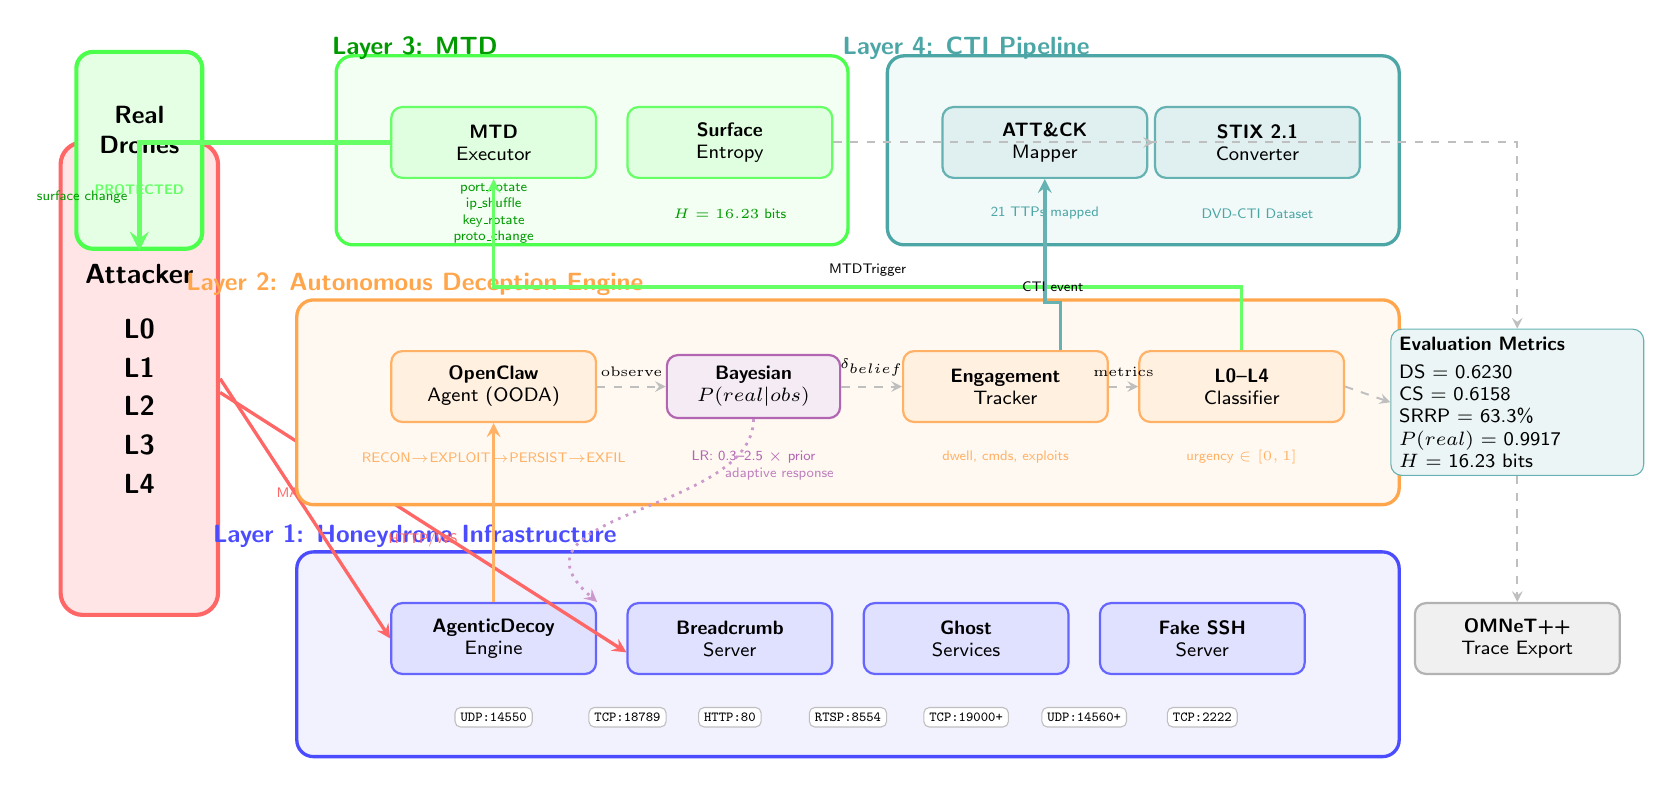
\begin{tikzpicture}[
    >=stealth,
    layer/.style={
        rectangle, rounded corners=6pt, draw=#1!70, fill=#1!5,
        line width=1.2pt, minimum height=2.8cm, align=center
    },
    comp/.style={
        rectangle, rounded corners=4pt, draw=#1!60, fill=#1!12,
        line width=0.8pt, minimum width=2.6cm, minimum height=0.9cm,
        align=center, font=\sffamily\scriptsize
    },
    port/.style={
        rectangle, rounded corners=2pt, draw=gray!50, fill=white,
        font=\ttfamily\tiny, inner sep=2pt
    },
    flow/.style={->, line width=1.2pt, draw=#1!60},
    dataflow/.style={->, line width=0.7pt, draw=gray!50, dashed},
    beliefbox/.style={
        rectangle, rounded corners=4pt, draw=violet!60, fill=violet!8,
        line width=0.8pt, font=\sffamily\scriptsize, align=center,
        minimum width=2.2cm, minimum height=0.8cm
    },
    metricbox/.style={
        rectangle, rounded corners=4pt, draw=teal!60, fill=teal!8,
        font=\sffamily\scriptsize, align=left, text width=3.0cm,
        inner sep=3pt
    },
]

% ═══════════════════════════════════════════════════════════════
% ATTACKER (left side)
% ═══════════════════════════════════════════════════════════════
\node[rectangle, rounded corners=8pt, draw=red!60, fill=red!10,
      line width=1.5pt, minimum width=2.0cm, minimum height=6cm,
      align=center, font=\sffamily\bfseries]
    (ATK) at (-2, 4.5) {Attacker\\[8pt]\romark{L0}\\[2pt]\romark{L1}\\[2pt]\romark{L2}\\[2pt]\romark{L3}\\[2pt]\romark{L4}};

% ═══════════════════════════════════════════════════════════════
% LAYER 1: Honeydrone Infrastructure (bottom)
% ═══════════════════════════════════════════════════════════════
\node[layer=blue, minimum width=14cm, minimum height=2.6cm] (L1) at (7, 1) {};
\node[font=\sffamily\bfseries\small, text=blue!70] at (1.5, 2.5) {Layer 1: Honeydrone Infrastructure};

% Components
\node[comp=blue] (engine) at (2.5, 1.2) {\textbf{AgenticDecoy}\\Engine};
\node[comp=blue] (bread)  at (5.5, 1.2) {\textbf{Breadcrumb}\\Server};
\node[comp=blue] (ghost)  at (8.5, 1.2) {\textbf{Ghost}\\Services};
\node[comp=blue] (ssh)    at (11.5, 1.2) {\textbf{Fake SSH}\\Server};

% Ports
\node[port] at (2.5, 0.2) {UDP:14550};
\node[port] at (4.2, 0.2) {TCP:18789};
\node[port] at (5.5, 0.2) {HTTP:80};
\node[port] at (7.0, 0.2) {RTSP:8554};
\node[port] at (8.5, 0.2) {TCP:19000+};
\node[port] at (10.0, 0.2) {UDP:14560+};
\node[port] at (11.5, 0.2) {TCP:2222};

% Attack arrows into Layer 1
\draw[flow=red] (ATK.east) -- node[above, font=\sffamily\tiny, text=red!60] {MAVLink} (engine.west);
\draw[flow=red] ([yshift=-5pt]ATK.east) -- node[below, font=\sffamily\tiny, text=red!60] {HTTP/WS} ([yshift=-5pt]bread.west);

% ═══════════════════════════════════════════════════════════════
% LAYER 2: Autonomous Deception (middle)
% ═══════════════════════════════════════════════════════════════
\node[layer=orange, minimum width=14cm, minimum height=2.6cm] (L2) at (7, 4.2) {};
\node[font=\sffamily\bfseries\small, text=orange!70] at (1.5, 5.7) {Layer 2: Autonomous Deception Engine};

\node[comp=orange] (ooda) at (2.5, 4.4) {\textbf{OpenClaw}\\Agent (OODA)};
\node[beliefbox]   (belief) at (5.8, 4.4) {\textbf{Bayesian}\\$P(\text{real}|\text{obs})$};
\node[comp=orange] (track) at (9.0, 4.4) {\textbf{Engagement}\\Tracker};
\node[comp=orange] (class) at (12.0, 4.4) {\textbf{L0--L4}\\Classifier};

% Subdetails
\node[font=\sffamily\tiny, text=orange!60] at (2.5, 3.5) {RECON$\to$EXPLOIT$\to$PERSIST$\to$EXFIL};
\node[font=\sffamily\tiny, text=violet!60] at (5.8, 3.5) {LR: 0.3--2.5 $\times$ prior};
\node[font=\sffamily\tiny, text=orange!60] at (9.0, 3.5) {dwell, cmds, exploits};
\node[font=\sffamily\tiny, text=orange!60] at (12.0, 3.5) {urgency $\in [0,1]$};

% Internal flows
\draw[flow=orange] (engine.north) -- (ooda.south);
\draw[dataflow] (ooda) -- node[above, font=\tiny] {observe} (belief);
\draw[dataflow] (belief) -- node[above, font=\tiny] {$\delta_{\text{belief}}$} (track);
\draw[dataflow] (track) -- node[above, font=\tiny] {metrics} (class);

% ═══════════════════════════════════════════════════════════════
% LAYER 3: MTD (top-left)
% ═══════════════════════════════════════════════════════════════
\node[layer=green, minimum width=6.5cm, minimum height=2.4cm] (L3) at (3.75, 7.4) {};
\node[font=\sffamily\bfseries\small, text=green!60!black] at (1.5, 8.7) {Layer 3: MTD};

\node[comp=green] (executor) at (2.5, 7.5) {\textbf{MTD}\\Executor};
\node[comp=green] (entropy) at (5.5, 7.5) {\textbf{Surface}\\Entropy};

\node[font=\sffamily\tiny, text=green!60!black, align=center] at (2.5, 6.6) {port\_rotate\\ip\_shuffle\\key\_rotate\\proto\_change};
\node[font=\sffamily\tiny, text=green!60!black] at (5.5, 6.6) {$H=16.23$ bits};

% MTD trigger from classifier
\draw[flow=green] (class.north) -- ++(0, 0.8) -| node[near start, above, font=\sffamily\tiny] {MTDTrigger} (executor.south);

% ═══════════════════════════════════════════════════════════════
% LAYER 4: CTI Pipeline (top-right)
% ═══════════════════════════════════════════════════════════════
\node[layer=teal, minimum width=6.5cm, minimum height=2.4cm] (L4) at (10.75, 7.4) {};
\node[font=\sffamily\bfseries\small, text=teal!70] at (8.5, 8.7) {Layer 4: CTI Pipeline};

\node[comp=teal] (parser) at (9.5, 7.5) {\textbf{ATT\&CK}\\Mapper};
\node[comp=teal] (stix)   at (12.2, 7.5) {\textbf{STIX 2.1}\\Converter};

\node[font=\sffamily\tiny, text=teal!70] at (9.5, 6.6) {21 TTPs mapped};
\node[font=\sffamily\tiny, text=teal!70] at (12.2, 6.6) {DVD-CTI Dataset};

% CTI flow
\draw[flow=teal] ([xshift=20pt]track.north) -- ++(0, 0.6) -| node[near start, above, font=\sffamily\tiny] {CTI event} (parser.south);
\draw[dataflow] (parser) -- (stix);

% ═══════════════════════════════════════════════════════════════
% METRICS OUTPUT (right side)
% ═══════════════════════════════════════════════════════════════
\node[metricbox] (metrics) at (15.5, 4.2) {
    \textbf{Evaluation Metrics}\\[2pt]
    DS = 0.6230\\
    CS = 0.6158\\
    SRRP = 63.3\%\\
    $P(\text{real})$ = 0.9917\\
    $H$ = 16.23 bits
};
\draw[dataflow] (class.east) -- (metrics.west);
\draw[dataflow] (entropy.east) -| (metrics.north);

% ═══════════════════════════════════════════════════════════════
% OMNeT++ Output (bottom-right)
% ═══════════════════════════════════════════════════════════════
\node[comp=gray] (omnet) at (15.5, 1.2) {\textbf{OMNeT++}\\Trace Export};
\draw[dataflow] (metrics.south) -- (omnet.north);

% ═══════════════════════════════════════════════════════════════
% REAL DRONES (protected, far left)
% ═══════════════════════════════════════════════════════════════
\node[rectangle, rounded corners=6pt, draw=green!70, fill=green!10,
      line width=1.5pt, minimum width=1.6cm, minimum height=2.5cm,
      align=center, font=\sffamily\bfseries\small]
    (REAL) at (-2, 7.4) {Real\\Drones\\[4pt]{\tiny\textcolor{green!60}{PROTECTED}}};

\draw[flow=green, line width=2pt] (executor.west) -| node[near end, left, font=\sffamily\tiny, text=green!60!black] {surface change} (REAL.south);

% ═══════════════════════════════════════════════════════════════
% Deception feedback loop (big curved arrow)
% ═════════════════════════════════════════════════════════���═════
\draw[->, line width=1pt, draw=violet!40, dotted]
    (belief.south) .. controls (5.8, 2.8) and (2.5, 2.8) .. (engine.north east)
    node[near start, right, font=\sffamily\tiny, text=violet!50] {adaptive response};

\end{tikzpicture}
}
\caption{MIRAGE-UAS 4-Layer 방어 아키텍처. 공격자 트래픽은 Layer~1의 허니드론 인프라에 유입되고, Layer~2의 자율 기만 엔진이 OODA 루프와 베이지안 믿음 추적으로 적응형 응답을 생성한다. Layer~3의 MTD는 공격자 레벨 기반 urgency에 따라 공격 표면을 재구성하며, Layer~4의 CTI 파이프라인은 공격 이벤트를 STIX 2.1 데이터셋으로 변환한다.}
\label{fig:defense}
\end{figure*}

% ═══════════════════════════════════════════════════════════════
\begin{figure*}[t]
\centering
\resizebox{\textwidth}{!}{%
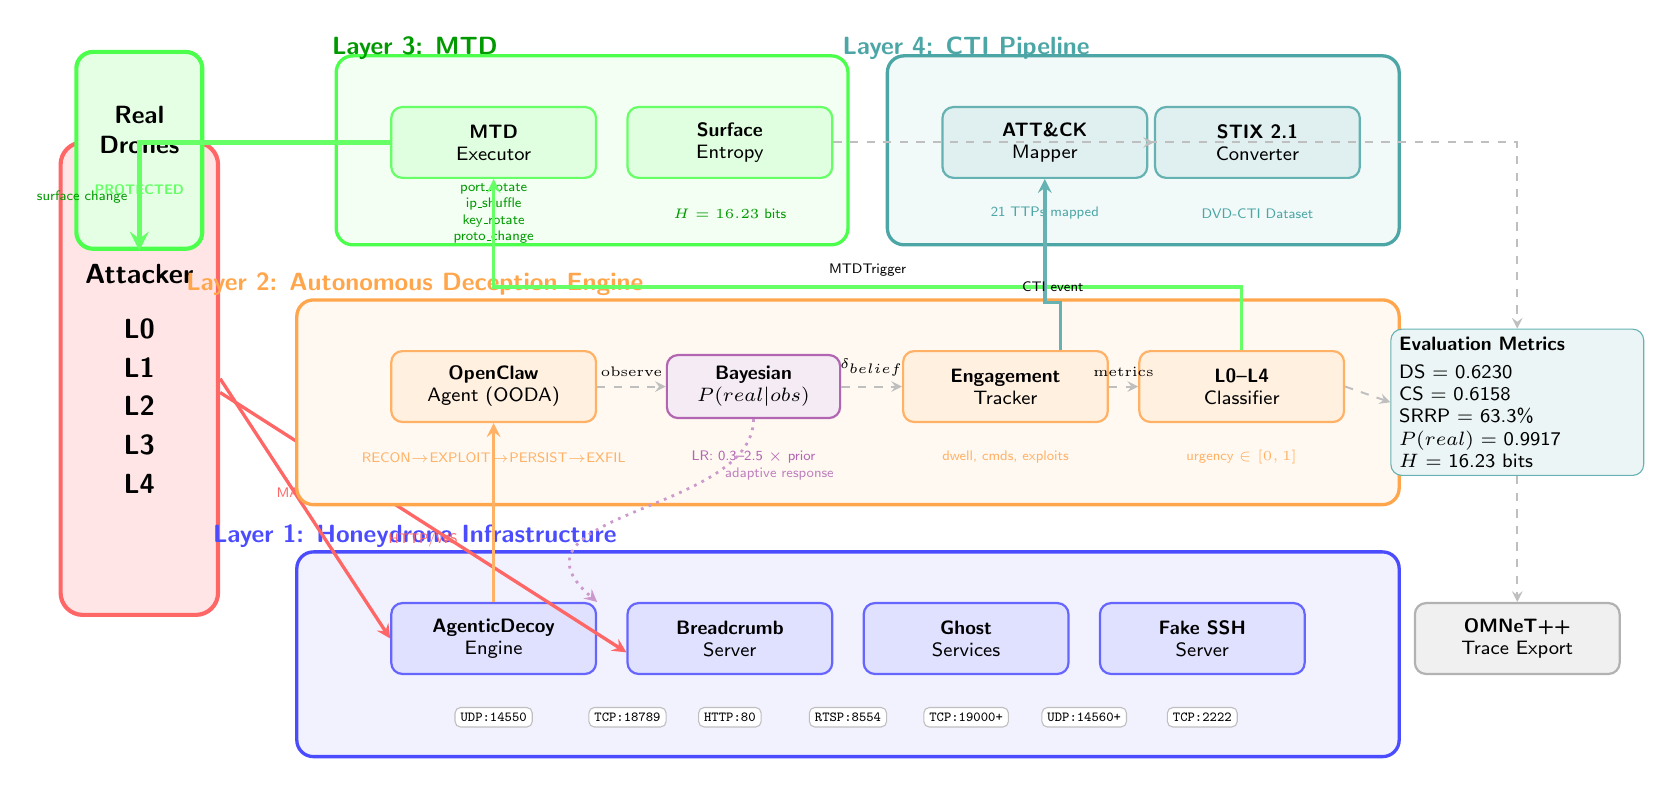
\begin{tikzpicture}[
    >=stealth,
    layer/.style={
        rectangle, rounded corners=6pt, draw=#1!70, fill=#1!5,
        line width=1.2pt, minimum height=2.8cm, align=center
    },
    comp/.style={
        rectangle, rounded corners=4pt, draw=#1!60, fill=#1!12,
        line width=0.8pt, minimum width=2.6cm, minimum height=0.9cm,
        align=center, font=\sffamily\scriptsize
    },
    port/.style={
        rectangle, rounded corners=2pt, draw=gray!50, fill=white,
        font=\ttfamily\tiny, inner sep=2pt
    },
    flow/.style={->, line width=1.2pt, draw=#1!60},
    dataflow/.style={->, line width=0.7pt, draw=gray!50, dashed},
    beliefbox/.style={
        rectangle, rounded corners=4pt, draw=violet!60, fill=violet!8,
        line width=0.8pt, font=\sffamily\scriptsize, align=center,
        minimum width=2.2cm, minimum height=0.8cm
    },
    metricbox/.style={
        rectangle, rounded corners=4pt, draw=teal!60, fill=teal!8,
        font=\sffamily\scriptsize, align=left, text width=3.0cm,
        inner sep=3pt
    },
]

% ═══════════════════════════════════════════════════════════════
% ATTACKER (left side)
% ═══════════════════════════════════════════════════════════════
\node[rectangle, rounded corners=8pt, draw=red!60, fill=red!10,
      line width=1.5pt, minimum width=2.0cm, minimum height=6cm,
      align=center, font=\sffamily\bfseries]
    (ATK) at (-2, 4.5) {Attacker\\[8pt]\romark{L0}\\[2pt]\romark{L1}\\[2pt]\romark{L2}\\[2pt]\romark{L3}\\[2pt]\romark{L4}};

% ═══════════════════════════════════════════════════════════════
% LAYER 1: Honeydrone Infrastructure (bottom)
% ═══════════════════════════════════════════════════════════════
\node[layer=blue, minimum width=14cm, minimum height=2.6cm] (L1) at (7, 1) {};
\node[font=\sffamily\bfseries\small, text=blue!70] at (1.5, 2.5) {Layer 1: Honeydrone Infrastructure};

% Components
\node[comp=blue] (engine) at (2.5, 1.2) {\textbf{AgenticDecoy}\\Engine};
\node[comp=blue] (bread)  at (5.5, 1.2) {\textbf{Breadcrumb}\\Server};
\node[comp=blue] (ghost)  at (8.5, 1.2) {\textbf{Ghost}\\Services};
\node[comp=blue] (ssh)    at (11.5, 1.2) {\textbf{Fake SSH}\\Server};

% Ports
\node[port] at (2.5, 0.2) {UDP:14550};
\node[port] at (4.2, 0.2) {TCP:18789};
\node[port] at (5.5, 0.2) {HTTP:80};
\node[port] at (7.0, 0.2) {RTSP:8554};
\node[port] at (8.5, 0.2) {TCP:19000+};
\node[port] at (10.0, 0.2) {UDP:14560+};
\node[port] at (11.5, 0.2) {TCP:2222};

% Attack arrows into Layer 1
\draw[flow=red] (ATK.east) -- node[above, font=\sffamily\tiny, text=red!60] {MAVLink} (engine.west);
\draw[flow=red] ([yshift=-5pt]ATK.east) -- node[below, font=\sffamily\tiny, text=red!60] {HTTP/WS} ([yshift=-5pt]bread.west);

% ═══════════════════════════════════════════════════════════════
% LAYER 2: Autonomous Deception (middle)
% ═══════════════════════════════════════════════════════════════
\node[layer=orange, minimum width=14cm, minimum height=2.6cm] (L2) at (7, 4.2) {};
\node[font=\sffamily\bfseries\small, text=orange!70] at (1.5, 5.7) {Layer 2: Autonomous Deception Engine};

\node[comp=orange] (ooda) at (2.5, 4.4) {\textbf{OpenClaw}\\Agent (OODA)};
\node[beliefbox]   (belief) at (5.8, 4.4) {\textbf{Bayesian}\\$P(\text{real}|\text{obs})$};
\node[comp=orange] (track) at (9.0, 4.4) {\textbf{Engagement}\\Tracker};
\node[comp=orange] (class) at (12.0, 4.4) {\textbf{L0--L4}\\Classifier};

% Subdetails
\node[font=\sffamily\tiny, text=orange!60] at (2.5, 3.5) {RECON$\to$EXPLOIT$\to$PERSIST$\to$EXFIL};
\node[font=\sffamily\tiny, text=violet!60] at (5.8, 3.5) {LR: 0.3--2.5 $\times$ prior};
\node[font=\sffamily\tiny, text=orange!60] at (9.0, 3.5) {dwell, cmds, exploits};
\node[font=\sffamily\tiny, text=orange!60] at (12.0, 3.5) {urgency $\in [0,1]$};

% Internal flows
\draw[flow=orange] (engine.north) -- (ooda.south);
\draw[dataflow] (ooda) -- node[above, font=\tiny] {observe} (belief);
\draw[dataflow] (belief) -- node[above, font=\tiny] {$\delta_{\text{belief}}$} (track);
\draw[dataflow] (track) -- node[above, font=\tiny] {metrics} (class);

% ═══════════════════════════════════════════════════════════════
% LAYER 3: MTD (top-left)
% ═══════════════════════════════════════════════════════════════
\node[layer=green, minimum width=6.5cm, minimum height=2.4cm] (L3) at (3.75, 7.4) {};
\node[font=\sffamily\bfseries\small, text=green!60!black] at (1.5, 8.7) {Layer 3: MTD};

\node[comp=green] (executor) at (2.5, 7.5) {\textbf{MTD}\\Executor};
\node[comp=green] (entropy) at (5.5, 7.5) {\textbf{Surface}\\Entropy};

\node[font=\sffamily\tiny, text=green!60!black, align=center] at (2.5, 6.6) {port\_rotate\\ip\_shuffle\\key\_rotate\\proto\_change};
\node[font=\sffamily\tiny, text=green!60!black] at (5.5, 6.6) {$H=16.23$ bits};

% MTD trigger from classifier
\draw[flow=green] (class.north) -- ++(0, 0.8) -| node[near start, above, font=\sffamily\tiny] {MTDTrigger} (executor.south);

% ═══════════════════════════════════════════════════════════════
% LAYER 4: CTI Pipeline (top-right)
% ═══════════════════════════════════════════════════════════════
\node[layer=teal, minimum width=6.5cm, minimum height=2.4cm] (L4) at (10.75, 7.4) {};
\node[font=\sffamily\bfseries\small, text=teal!70] at (8.5, 8.7) {Layer 4: CTI Pipeline};

\node[comp=teal] (parser) at (9.5, 7.5) {\textbf{ATT\&CK}\\Mapper};
\node[comp=teal] (stix)   at (12.2, 7.5) {\textbf{STIX 2.1}\\Converter};

\node[font=\sffamily\tiny, text=teal!70] at (9.5, 6.6) {21 TTPs mapped};
\node[font=\sffamily\tiny, text=teal!70] at (12.2, 6.6) {DVD-CTI Dataset};

% CTI flow
\draw[flow=teal] ([xshift=20pt]track.north) -- ++(0, 0.6) -| node[near start, above, font=\sffamily\tiny] {CTI event} (parser.south);
\draw[dataflow] (parser) -- (stix);

% ═══════════════════════════════════════════════════════════════
% METRICS OUTPUT (right side)
% ═══════════════════════════════════════════════════════════════
\node[metricbox] (metrics) at (15.5, 4.2) {
    \textbf{Evaluation Metrics}\\[2pt]
    DS = 0.6230\\
    CS = 0.6158\\
    SRRP = 63.3\%\\
    $P(\text{real})$ = 0.9917\\
    $H$ = 16.23 bits
};
\draw[dataflow] (class.east) -- (metrics.west);
\draw[dataflow] (entropy.east) -| (metrics.north);

% ═══════════════════════════════════════════════════════════════
% OMNeT++ Output (bottom-right)
% ═══════════════════════════════════════════════════════════════
\node[comp=gray] (omnet) at (15.5, 1.2) {\textbf{OMNeT++}\\Trace Export};
\draw[dataflow] (metrics.south) -- (omnet.north);

% ═══════════════════════════════════════════════════════════════
% REAL DRONES (protected, far left)
% ═══════════════════════════════════════════════════════════════
\node[rectangle, rounded corners=6pt, draw=green!70, fill=green!10,
      line width=1.5pt, minimum width=1.6cm, minimum height=2.5cm,
      align=center, font=\sffamily\bfseries\small]
    (REAL) at (-2, 7.4) {Real\\Drones\\[4pt]{\tiny\textcolor{green!60}{PROTECTED}}};

\draw[flow=green, line width=2pt] (executor.west) -| node[near end, left, font=\sffamily\tiny, text=green!60!black] {surface change} (REAL.south);

% ═══════════════════════════════════════════════════════════════
% Deception feedback loop (big curved arrow)
% ═════════════════════════════════════════════════════════���═════
\draw[->, line width=1pt, draw=violet!40, dotted]
    (belief.south) .. controls (5.8, 2.8) and (2.5, 2.8) .. (engine.north east)
    node[near start, right, font=\sffamily\tiny, text=violet!50] {adaptive response};

\end{tikzpicture}
}
\caption{MIRAGE-UAS 4-Layer 방어 아키텍처. 공격자 트래픽은 Layer~1의 허니드론 인프라에 유입되고, Layer~2의 자율 기만 엔진이 OODA 루프와 베이지안 믿음 추적으로 적응형 응답을 생성한다. Layer~3의 MTD는 공격자 레벨 기반 urgency에 따라 공격 표면을 재구성하며, Layer~4의 CTI 파이프라인은 공격 이벤트를 STIX 2.1 데이터셋으로 변환한다.}
\label{fig:defense}
\end{figure*}
